\chapter{Testování}
\label{ch:testing}
Je několik různých typů testů, které se navzájem doplňují nebo překrývají. V rámci této práce byly vytvořeny automatické testy jednotkové a integrační a to za pomoci nástroje \nameref{ss:jest}. V následujících sekcích se podíváme právě na jednotkové a integrační testy, na další možnosti testování a na finální zhodnocení aplikace a budoucí vývoj.

\section{Jednotkové testy}
\label{sc:unit_tests}
Jednotkový test je typ testu, který testuje jednotlivé třídy, metody a funkce nezávisle na zbytku aplikace. Jak již bylo zmíněno v sekci \nameref{ss:clean_architecture}, rozdělení na vrstvy ulehčí testování. V rámci práce jsou takto testovány intereactory, které provádí změny nad entitami. Tím je zajištěno že všechny operace s entitami a to jak na backendu, tak na frontendu jsou validní.

\section{Integrační testy}
\label{sc:unit_tests}
Na rozdíl od jednotkového testu, který testuje jednotlivé nezávislé funkce čí metody, tak test integrační testuje více částí aplikace najednou. Zjistí se tím funkčnost celého systému. Bohužel, kvůli volbě verzi \nameref{ss:yarn} nebylo možné správně nakofigurovat řádný integrační test. První pokus bylo rozšíření pro \nameref{ss:storybook} \emph{storyshots}, který při spuštění vytvoří obrázky daných komponent a při dalších spuštěních je srovnává s předchozí verzí a případně notifikuje vývojáře. Další pokus byla konfigurace knihovny \emph{Cypress}, která umožňuje vytvářet \acrfull{e2e} testovací scénáře, které simulují průchody aplikací. Oba pokusy selhaly kvůli špatné integraci knihovny \emph{babel}, která transpiluje typescriptové soubory na soubory javascriptové a vytváří cesty k externím knihovnám, což byl práě důvod neúspěchu.

\section{Ostatní testy}
Samozřejmě existuje více druhů testů než pouze \hyperref[sc:unit_tests]{jednotkové} a \hyperref[sc:unit_tests]{integrační}. V rámci této práce by nás mohli zajímat hlavně testy akceptační a smoke. Akceptační test je v pravém slova smysl test klientem kterému předáváme software. V rámci této práce by se za akceptační test dal považovat test uživateli, který ale nemohl být uskutečněn a to kvůli absenci dat. Smoke testy jsou testy nasazení. Po nasazení se spustí jednoduchá testovací sada, která má za úkol ověřit zdali se aplikace správně nasadila a odpovídá.

\section{Budoucí vývoj}
\label{sc:upcomming_development}
Aplikace je nyní ve fázi funkčního prototypu, jsou implementovány všechny základní požadavky, ale stále je zde prostor na zlepšení. V následujících sekcích jsou rozebrány některé takové faktory.

\subsection{Doprání testů}
Asi největším nedostatkem aplikace je absence \hyperref[sc:unit_tests]{integračních testů}, což koncového uživatele může, ale nemusí postihnout. Tento nedostatek půjde vyřešit ve chvíli, kdy vývojáři babelu plně dokončí integraci nové verze yarnu. Do té doby bohužel není možnost takové testy psát, protože všechny testovací frameworky, které umožňují více než jen jednotkové testy, na této knihovně závisí.

\subsection{Data}
To co nejvíce aplikaci schází v tuto dobu jsou funkční data. Tím jsou myšleny písně s texty, akordy atd. Tyto data se dají jednoduše najít, ale pro osobní použití. Bohužel není žádné API poskytující seznam písní s textem a akordy pro ukulele. Tato data by se dala získat buď přepisem z jiných stránek či jejich scrapovaním, což by už mělo přesah do autorského zákona. Další možnost je kontaktovat přímo vydavatele a uzavřít spolupráci, která avšak nejspíš bude velmi finančně náročná. Poslední možnost by byla uzavřít spolupráci s již existujícímí aplikacemi a získat data od nich.

\subsection{Úpravy aplikace}
Hlavním neduhem stávající aplikace je hlavně design. Aplikace je sice ve dvou barevných schématech, ty však nejsou zcela vyladěné. Samotná úprava barev a rozložení nebude náročná, díky dělení na komponenty a použití globálně dostupných barevných schémat. Zároveň je možné v budoucnu přidat další barevná schémata na vrch dvou stávajících.

\subsection{Překlad}
Důležitou součástí aplikace, která míří na mezinárodní trh, tak je co největší jazyková dostupnost. Další krokem úpravy aplikace by tedy mělo být překlad do dalších jazyků, pro přilákání co největší skupiny uživatelů.

\subsection*{Podpora vybrnkávání}
Vybrnkávání je styl hraní na ukulele, kde se nehraje přejíždněním přes všechny struny, ale o některé se brnká. Tento styl má uplně jiný styl zobrazení. Jsou zobrazeny jednotlivé struny a k nim čísla pražců. Tato čísla jsou rozdělena do sloupců, které odpovídají době. Příklad takové tablatury je na obrázku \ref{fig:tablature}

\begin{figure}[h!]
    \centering
    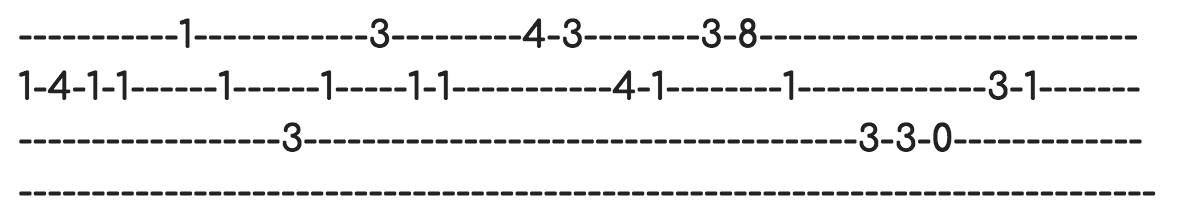
\includegraphics[width=\textwidth]{assets/picking.png}
    \caption{Noty pro vybrnkávání}
    \label{fig:tablature}
\end{figure}

\subsection*{Nastavení ladění}
Tato funkcionalita je témeř imlementována. Komponenta vykreslovaného akordu dostává na vstupu mimo akordu k vykreslení i aktuální ladění, které je vždy nastaveno na \emph{gcea}. Rozšíření by tedy spočívalo v přidání možnosti uživateli si toto ladění změnit, případně uložit pro příští návštěvy.

